\newpage
\chapter{Additional improvements}

Since we observed that the computation time to solve hard instances significantly increased compared to easy instances, we decided to implement the improvements described in chapters 4 and 5 of Calik and Tansel (2013), i.e. the ``BINARY'' and ``Double bound'' algorithms.\\\\
Let: 
\begin{itemize}
	\item LPx denote the relaxation of Px
	\item val(LPx) denote the optimal value of Px.
	\item RPx denote the relaxation that retain the objective function and all constraints of Px
\end{itemize} 

\section{BINARY algorithm}

Let:
\begin{itemize}
	\item $P_h$ with $h \in T$ be the problem P3 with the additional constraint $z_h = 1$
	\item $RP_h$ with $h \in T$ be the problem RP3 with the additional constraint $z_h = 1$
	\item val($P_h$) be the optimal value of $P_h$
	\item val($RP_h$) be the optimal value of $RP_h$
\end{itemize}\ \\
Calik and Tansel (2013) proposes and proves that val($RP3$)$ = \min_{h \in T}$ val($RP_h$). They show that computing $\min_{h \in T}$ val($RP_h$) is achieved in polynomial time by solving $\mathcal{O}\left( \log_2 K \right)$ linear programs $RP_h$ for each $\rho_h$ selected from the set of ordered $\rho$ values $R = \lbrace \rho_1, \rho_2, ..., \rho_K \rbrace$ (as defined in P3) during a binary seach.\\\\
The BINARY algorithm proposed by Calik and Tansel (2013) can be schematized as follows:
\begin{figure}[H]
	\begin{center}
		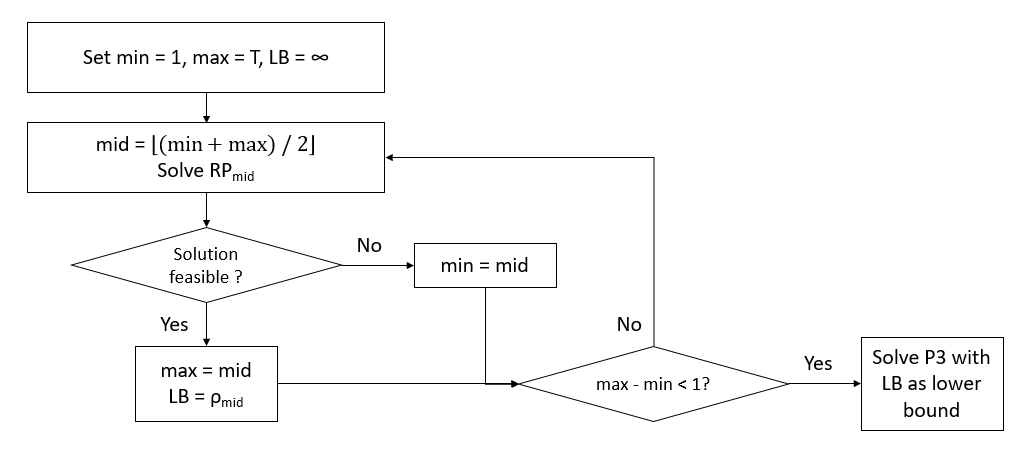
\includegraphics[width=\textwidth]{../imgs/BINARY.png}
		\caption{Flow chart of BINARY algorithm}
	\end{center}
\end{figure}

\section{Double bound algorithm}

Let:
\begin{itemize}
	\item $S$ be any nonempty subset of $T = \lbrace 1, ..., K \rbrace$
	\item $P(S)$ be the problem which is exactly the same as P3 except that all variables $z_k, k \in T\\S$ are dropped from P3
\end{itemize}\ \\
Calik and Tansel (2013) proposes and proves the following:\\\\
``Suppose $|S| > 2$. Let a and b be the smallest ad largest indices in S, respectively.\\
\begin{tabularx}{\textwidth}{l X}
(a) & If val($P(S)$) = $\rho_a$, then $r_p(F) \in \lbrace \rho_1, ..., \rho_a \rbrace$\\
(b) & If val($P(S)$) = $\rho_k$ for some $k$ with $a < k \leq b$, then $r_p(F) \in \lbrace \rho_{k'+1}, ..., \rho_k \rbrace$ where $k'$ is the largest index in $S$ which is smaller than $k$ \\
(c) & If val($P(S)$) = $\infty$, then $r_p(F) \in \lbrace \rho_{b+1}, ..., \rho_K \rbrace$''\\
\end{tabularx}\ \\\\
This proposition allows the construction of a more efficient search strategy based on the restriction of P3. The Double bound algorithm proposed by Calik and Tansel (2013) is based on this proposition and can be schematized as follows:
\begin{figure}[H]
	\begin{center}
		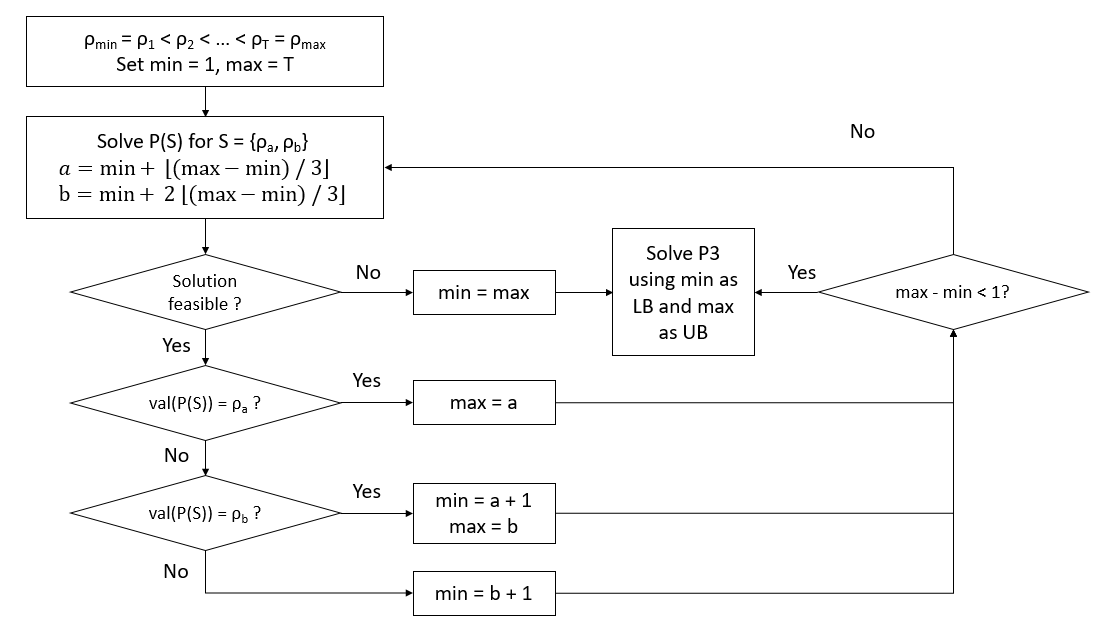
\includegraphics[width=\textwidth]{../imgs/DB3.png}
		\caption{Flow chart of DB3 algorithm}
	\end{center}
\end{figure}